\documentclass{article}
\title{Math 120 Assignment 1}
\author{Isaac Winger 20167000}
\date{}
\pagenumbering{gobble}

\usepackage{graphicx}
\usepackage{amsfonts}
\graphicspath{ {./} }

\begin{document}
    \begin{enumerate} \addtocounter{enumi}{2}
      \item \begin{enumerate}
                    \item $ \lbrack a,b \rbrack = \{x \in \mathbb{R} \mid a \leq x \leq b\} $ \\
                    $ \lbrack c,d \rbrack = \{x \in \mathbb{R} \mid c \leq x \leq d\} $

                    \item Since $x \in \lbrack a,b \rbrack$, using the set build form above it can be converted to $a \leq x \leq b$. Then, simplify this statement into $x \leq b$. Using the premise of $b \leq d$, it is known that $x \leq b \leq d$. Once again, this can be simplified to $x \leq d$, resulting in the desired statement.

                    \item Since $b \in \lbrack a,b \rbrack$, from the premise that $\lbrack a,b \rbrack \subseteq \lbrack c,d \rbrack$ and the fact that any element of a subset must also exist in the superset, it is known that $b \in \lbrack c,d \rbrack$. From the set build form above, this implies that $c \leq b \leq d$. This can be simplified to show that $b \leq d$, demonstrating the desired statement.

                    \item \begin{figure}[h]\centering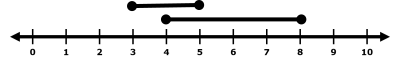
\includegraphics[width=3in]{numline}\end{figure} \vspace{-10ex}

                    \vspace{5ex}\item No, for example $3 \in \lbrack 3,5 \rbrack$, but it's also the case that $3 \notin \lbrack 4,8 \rbrack$. So by definition of a subset, there is an element that exists in $\lbrack 3,5 \rbrack$ that doesn't exist in $\lbrack 4,8 \rbrack$, so $\lbrack 3,5 \rbrack \not\subseteq \lbrack 4,8 \rbrack$.

              \item In this case $b \leq d$, but $a \not\leq c$.

                    \item \begin{figure}[h]\centering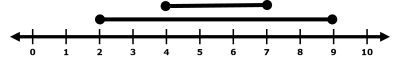
\includegraphics[width=3in]{numline2}\end{figure} \vspace{-10ex}

                    \vspace{5ex}\item Yes, as can be seen in the example above every element of $\lbrack 4,7 \rbrack$ exists in $\lbrack 2,9 \rbrack$.

                    \item Since $\lbrack 4, 7 \rbrack \subseteq \lbrack 2,9 \rbrack$, both statements should be true based on the proof above.
                    \end{enumerate}
    \end{enumerate}

\end{document}
